\section{Matplotlib} % (fold)
\label{sec:matplotlib}
\begin{questions}
\titledquestion{Plotting a function} % (fold)
\label{sub:plotting_a_function}

Plot the function
\[
    f(x) = \sin^2(x-2)e^{-x^2}
\]
over the interval $[0,2]$.
Add proper axis labels, a title, etc.

% titledquestion plotting_a_function (end)

\titledquestion{Data} % (fold)
\label{sub:data}

Create a data matrix $X$ with 20 observations of 10 variables.
Generate a vector $b$ with parameters
Then generate the response vector $y = Xb + z$ where $z$ is a vector with
standard normally distributed variables.

Now (by only using y and X), find an estimator for $b$, by solving
\[
    \hat b = \arg\min_b \|Xb - y\|_2
\]

Plot the true parameters $b$ and estimated parameters $\hat b$.
See Figure~\ref{fig:param_plot} for an example plot.

\begin{figure}
    \centering
    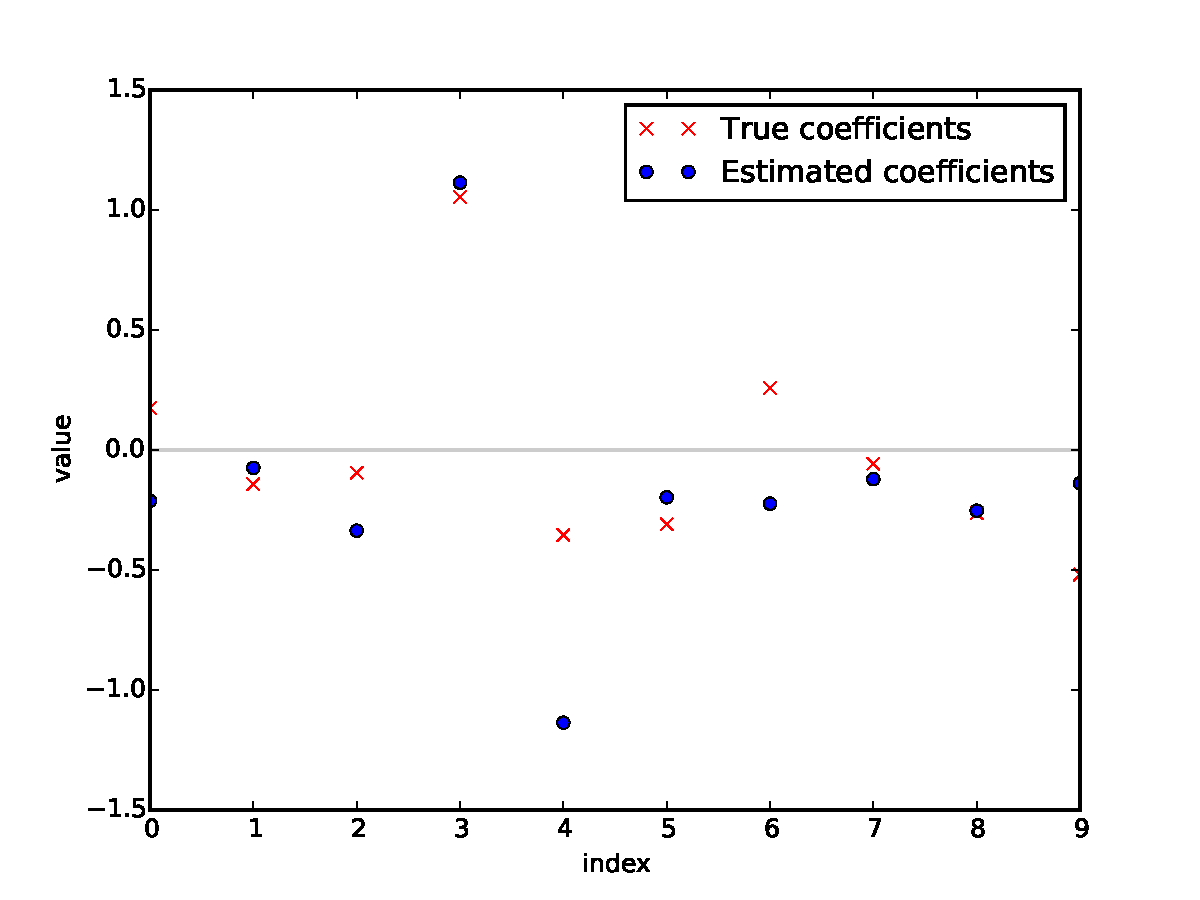
\includegraphics[width=.45\textwidth]{img/param_plot.pdf}
    \caption{Parameter plot}
    \label{fig:param_plot}
\end{figure}

% titledquestion data (end)

\titledquestion{Histogram and density estimation} % (fold)
\label{sub:histogram_and_density_estimation}

Generate a vector $z$ of $10000$ observations from your favorite exotic distribution.
Then make a plot that shows a histogram of $z$ (with 25 bins), along with an estimate for the density,
using a Gaussian kernel density estimator (see scipy.stats).
See Figure~\ref{fig:hist} for an example plot.

\begin{figure}
    \centering
    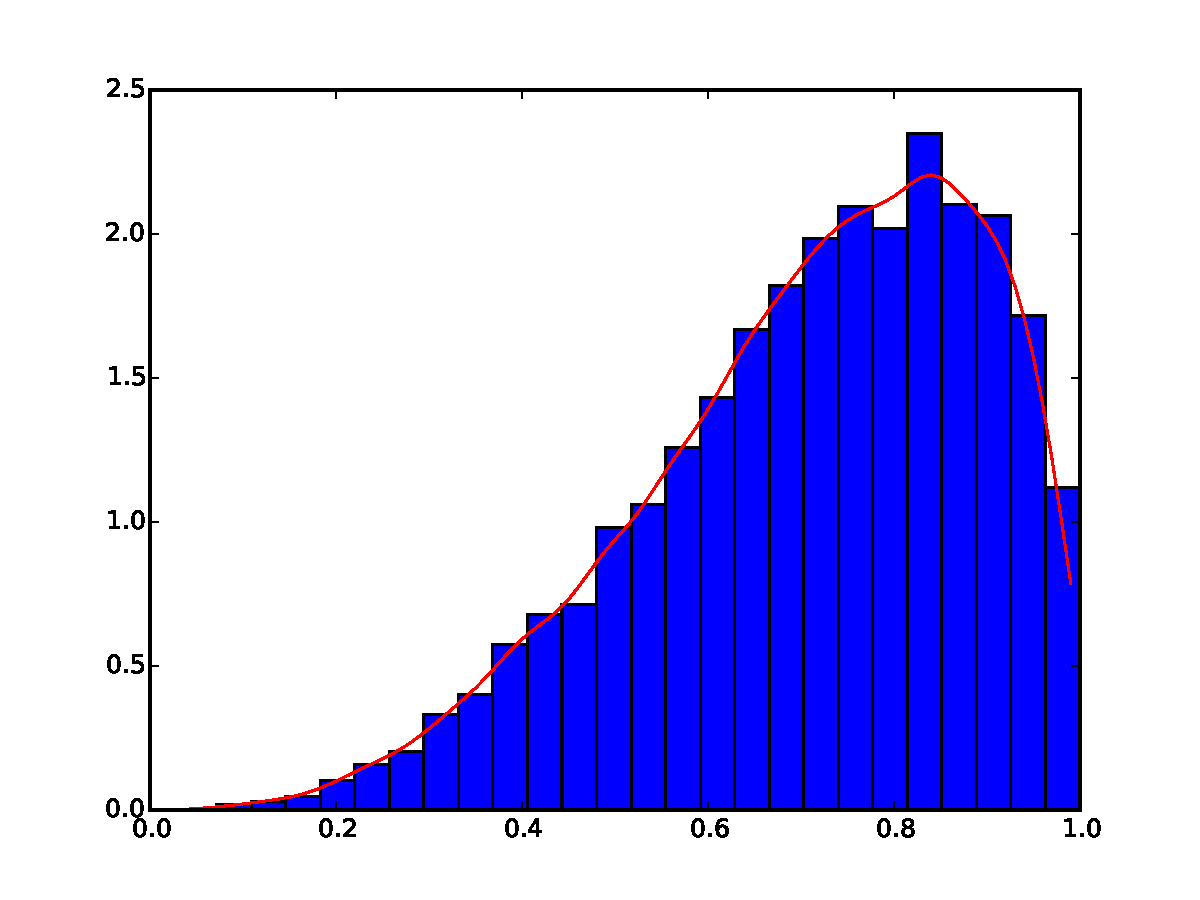
\includegraphics[width=.45\textwidth]{img/hist_plot.pdf}
    \caption{Histogram}
    \label{fig:hist}
\end{figure}

% titledquestion histogram_and_density_estimation (end)
\end{questions}
% section matplotlib (end)
